%% Benutzerdefinierte Kommandos

	\newcommand{\todo}[1]{\colorbox{red}{\textcolor{white}{TODO: #1}}}
	


%% Pakete 

\documentclass[a4paper, 12pt]{scrartcl}
\usepackage{ucs}
\usepackage[utf8x]{inputenc}
\usepackage[T1]{fontenc}
\usepackage[english,ngerman]{babel}
\usepackage{graphicx}
\usepackage{enumerate}
\usepackage{color}
\usepackage{xcolor}
\usepackage{amsfonts}
\usepackage{amsmath}
\usepackage{scrtime} % for \thistime
\usepackage{dsfont} %for \mathds
\usepackage{framed}
\usepackage[colorlinks=true,urlcolor=blue,linkcolor=black]{hyperref}
\usepackage{perpage} %the perpage package, used for footnotes
\usepackage{pifont} %used for customized footnotes
\usepackage{caption}
\usepackage{float}
\usepackage{mathrsfs}
\usepackage[usestackEOL]{stackengine}



\begin{document}

\begin{normalsize}

\raggedright\textbf{\Huge Peketeinräumerding}\\	
		\begin{flushright}
		\textit{...}
		\textit{...}
		\textit{...}
		\textit{Felix Baral-Weber}\\
		Stand: \space \today \space \thistime
		\end{flushright}

\end{normalsize}

\section{Einführung}
\subsection{Zweck des Dokuments}
Dieses Dokument beschreibt die Anforderungen und Implementierungsdetails an eine Echtzeitsystemanwendung die das Abschlussprojekt des Moduls Echtzeitbetriebssysteme der EAH Jena. Dieses Dokument richtet sich dabei an den Vorgaben für ein Software Requirements Specification (SRS) nach dem \href{https://de.wikipedia.org/wiki/Software_Requirements_Specification}{IEEE Standard 830-1998}. Der Modulverantwortliche ist Prof Dr. Oliver Jack aus dem Fachbereich Elektrotechnik und Informationstechnik.\\

\subsection{Einstieg in die Projektphase}
Die Arbeit an der Programmumsetzung wurde in die Teilbereiche Hochregal-Steuerung, Simulation, Integritätsprüfung und User-Input und Visualisierung aufgeteilt um diese Bereiche allein bzw. in Gruppen parallel  abarbeiten zu können.\\
Dabei ergab sich folgende Aufteilung:
\begin{itemize} 
	\item Hochregal-Steuerung $\rightarrow$ Michael Thomas, Simon Weitzel
	\item Simulation $\rightarrow$ Felix Baral-Weber, Andreas Glatz
	\item Integritätsprüfung und User-Input $\rightarrow$ Simon Weitzel, Michael Thomas
	\item Visualisierung $\rightarrow$ Andreas Glatz, Felix Baral-Weber
\end{itemize}

Desweiteren wurden Hauptverantwortliche für alle Teilbereich des Projekt festgelegt.\\

Die da wären:\\
\begin{itemize} 
	\item Michael Thomas: Programmumsetzung
	\item Andreas Glatz: Tests
	\item Simon Weitzel: Strukturierte Analyse
	\item Felix Baral-Weber: Latex-Template und Funktionale Anforderung
\end{itemize}
\section{Allgemeine Beschreibung}

\section{Spezifische Anforderungen}
\subsection{Funktionale Anforderungen}
\subsubsection{DFD1 Simulation}
\begin{figure}[H]
	\centering
  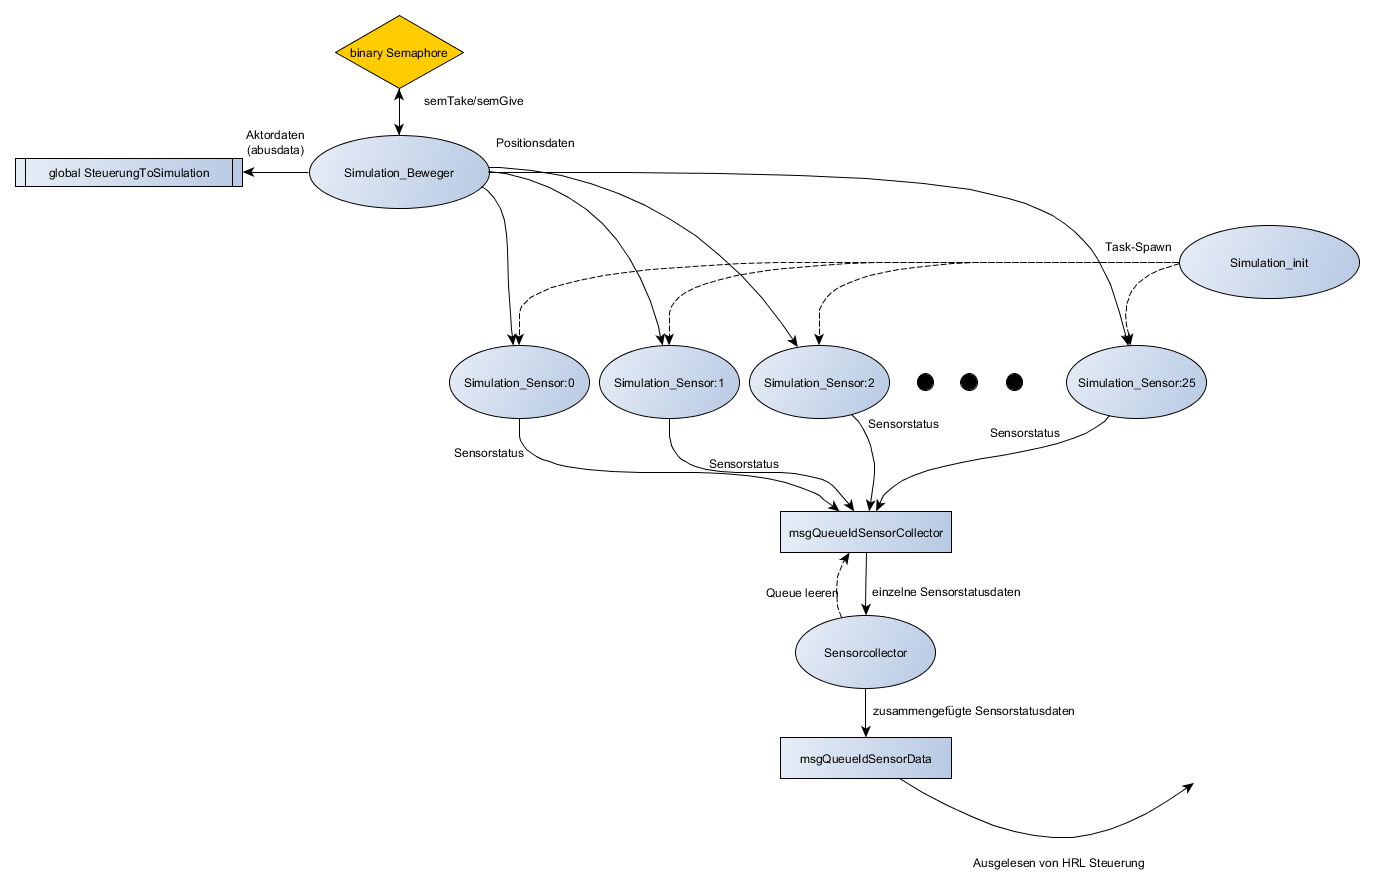
\includegraphics[width=\textwidth]{DFD/dfd1_simulation1_1.png}
	\caption{DFD1 Simulation}
	\label{fig1}
\end{figure}
\begin{figure}[H]
	\centering
  \includegraphics[width=\textwidth]{diagrams/gand.png}
	\caption{Gantt Diagramm der Task der Simulation}
	\label{gantt}
\end{figure}
\paragraph{Sensorcollector}
Der \textbf{Sensorcollector} sammelt aus der \textbf{MessageQueue} die Einträge aller Sensoren. Wenn ein Sensor ausfällt bleibt der Wert des Sensors auf 1.
%\input{lectures/lecture12}
\end{document}